\section{Experiments}
\label{sec:experiments}

\subsection{Experimental Setup}

\subsubsection{Dataset}
\label{subsec:datasets}
As described in Sec~\ref{sec:paired_dataset}, a high-quality dataset that pairs sign language with speech containing prosodic information does not currently exist. Therefore, we train our model using the two unimodal datasets described below.

\noindent{\bf OpenASL}~\cite{shi-etal-2022-open} is a large-scale American Sign Language (ASL) and text dataset collected from YouTube.
It contains diverse situational sign language videos It contains 98,417 translation pairs,
making it one of the largest publicly available ASL translation datasets. 
% In our experiments, we narrowed the set to 16,275 pairs for training simply to examine whether sign prosody is reflected in speech synthesis. 
For our experiments, we subsampled 16,275 pairs for training to evaluate the feasibility of reflecting sign prosody in speech synthesis.
The validation and test sets are composed of 961 and 970 pairs, respectively.

\noindent{\bf VCTK}~\cite{VCTK} is an English speech dataset recorded in a studio by 109 speakers. 
% Each speaker reads different texts; however, some texts are read by multiple speakers. 
We use this dataset as real speech data for adversarial learning.
The total duration of audio exceeds 44 hours, recorded at 48 kHz and converted to 16-bit.

\vspace{-2mm}
\subsubsection{Dataset Preprocessing}
Sign language videos were processed with MMPose~\cite{mmpose} to extract keypoints, and then we clipped the input video frame lengths to be between 30 and 512 frames. To exclude sign language samples with excessively long text, we removed those that deviated by more than 10 standard deviations from the mean.
% The keypoints consist of the wrist, fingertips, elbows, shoulders, and face, yielding $x$ and $y$ coordinates for each part.
For the audio, we used the Montreal Forced Aligner~\cite{mfa} to obtain 80-dimensional mel-spectrograms with a frame size of 1024 and hop size of 256.

\vspace{-2mm}
\subsubsection{Network Details}
Our model is based on FastSpeech2 and was pretrained on VCTK to acquire speaker information. We utilized open-source implementations of FastSpeech2\footnote{\url{https://github.com/ming024/FastSpeech2}} and the Visual Backbone\footnote{\url{https://github.com/HenryLittle/GloFE}}.
% The Prosody Estimator is composed of an FCN and prediction heads for each prosody label.
We trained our model on 3 NVIDIA RTX A5000 GPUs with a per-GPU batch size of 10.
For the optimization method, we used AdamW~\cite{loshchilov2018decoupled} for all models. For more details regarding hyper parameters and model implementation, please refer to the Appendix.

\vspace{-2mm}
\subsubsection{Evaluation Method}
In this paper, we evaluate the quality of synthesized speech using both objective and subjective assessments.
For the objective evaluation, 
we measure the expressiveness and naturalness of synthesized speech. 
For subjective evaluation, 
we conduct a user study and report comparative mean opinion scores (CMOS),
\manabe{following previous work of cross-lingual prosody transfer~\cite{swiatkowski23_interspeech}.}

\noindent{\bf Expressiveness}
To measure the richness of emotional expression in speech,
we calculate the standard deviations of predicted pitch and energy contours. 
Larger standard deviations indicate richer emotional expression~\cite{kharitonov-etal-2022-text}.
To evaluate the overall speech quality, 
we calculate the standard deviation across the test set, 
and to evaluate individual samples, 
we calculate the standard deviation for each speech sample and then take the mean of these values.

\noindent{\bf Naturalness}
To evaluate the quality of the synthesized speech and to show that our model does not degrade the quality of the speech, 
we use WER (Word Error Rate) and UTMOS\footnote{\url{https://github.com/sarulab-speech/UTMOS22}}~\cite{saeki22c_interspeech}. 
We use the pretrained automatic speech recognition model, 
Whisper large V3\footnote{\url{https://huggingface.co/openai/whisper-large-v3}}~\cite{radford2022whisper} to calculate WER. 
In particular, some text translations in OpenASL are inappropriate for speech synthesis: too long texts or too rare vocabularies. 
Therefore, we filtered out the text longer than 18 words and the text containing words of three or more capital letters.

\noindent{\bf User Study}
% We conducted a CMOS test to compare the two-stage method with the proposed method in how well the synthesized speech matches the source sign language prosody and naturalness. 
\manabe{
We conducted a CMOS test to evaluate how well and naturally
the synthesized speech matches the source sign language prosody. 
}
We grouped samples into three categories based on text length: Short (3-8 words), Medium (9-13 words), and Long (14-18 words). 
In addition, we categorized the 30 sign language videos with the lowest mean facial velocity as Neutral. 
% When the sign language contains low prosody, 
% the two-stage method can still produce speech with adequate prosody. 
% Therefore, on low prosody samples, 
% SignRecGAN should simply avoid degrading speech quality.
Given that the two-stage approach yields sufficient prosody, SignRecGAN's primary role in these cases is to maintain baseline speech quality without introducing artifacts.
In the CMOS test, 17 participants\footnote{A participant accidentally took the two types of tests.} rated each sample on a five grade evaluation.
Please refer to the Appendix for more details on the user study.

\noindent{\bf Prominence Analysis}
While our proposed method primarily focuses on reconstructing global prosody, it is crucial to verify whether this also results in high-quality, fine-grained prosodic features. 
To this end, we conducted a prominence analysis using the Wavelet Prosody Toolkit\footnote{\url{https://github.com/asuni/wavelet_prosody_toolkit}}~\cite{DBLP:journals/corr/SuniAV15}. For a more detailed explanation of prominence analysis,
please refer to the Appendix.

\begin{table}[t]\fontsize{10pt}{10pt}\selectfont
    \centering
    \caption{Objective evaluation. 
    % Expressiveness is considered better the closer its values to those of real speech. 
    The best scores are highlighted in \textbf{bold}, and the second-best scores are \underline{underlined}.}
    \label{tab:objective}
    \vspace{-3mm}
    \begin{tabular}[t]{lccccccc}
    \toprule
      &&&& \multicolumn{2}{c}{Expressiveness} & \multicolumn{2}{c}{Naturalness} \\
    Method & $\mathcal{L}_{\mathrm{natural}}$ & $\mathcal{L}_{\mathrm{SignRec}}$ & $\mathcal{L}_{\mathrm{ProMo}}$ & Pitch($\rightarrow$) & Energy($\rightarrow$) & WER($\downarrow$) & UTMOS($\uparrow$) \\
    \midrule
    Real Speech &  &  &  & 28.9 & 25.4 & 0.04 & 4.07 \\
    \midrule
    two-stage &  &  &  & \underline{17.6} & 20.1 & \underline{0.293} & \textbf{3.52} \\
    \midrule
    \multirow{4}{*}{Ours} & \Checkmark &  &  & 48.4 & 44.6 & \textbf{0.212} & 3.29 \\
     & \Checkmark & \Checkmark &  & 44.2 & 39.7 & 0.448 & 2.95 \\
     & \Checkmark &  & \Checkmark   & 45.3 & \underline{28.6} & 0.623 & 3.03 \\
     & \Checkmark & \Checkmark & \Checkmark                  & \textbf{33.7} & \textbf{22.5} & 0.325 & \underline{3.44}\\
    \bottomrule
    \end{tabular}
    \vspace{-4mm}
\end{table}


\subsection{Objective Evaluation}
Table~\ref{tab:objective} shows the result of comparing the expressiveness of the synthesized speech and that of real speech. 
As can be seen, SignRecGAN exhibits higher expressiveness values for pitch and energy than the two-stage method, 
and these values are closer to those of real speech. 
This suggests that intonation and emphasis similar to real speech can be achieved more effectively than with the two-stage method, 
although SignRecGAN slightly degrades the naturalness of the synthesized speech compared to the two-stage method.

\subsection{Ablation Study}
To investigate the effectiveness of each component in SignRecGAN, we conducted an ablation study.
GAN, SignRec, and ProMo indicate the S2PFormer with the losses defined in Eqs.~\ref{eq:natural}, \ref{eq:sign_rec}, \ref{eq:pro_mo} respectively.
The result in Table~\ref{tab:objective} show that every component alone does not contribute to improvement of expressiveness, and the combination of all three components is necessary to achieve the best performance. 
In particular, our ablation shows that 
if either the SignRec loss or the ProMo loss is removed, 
naturalness degrades even with the adversarial loss, 
indicating that all three components are necessary to maintain natural-sounding speech.
% Especially, the combinations of GAN with SignRec loss and with ProMo loss show significant degradation in naturalness.

\begin{table}[t]
    \centering
    \caption{The CMOS of the user study with 95\% confidence intervals. The scores with statistically significant improvements are highlighted in \colorbox{lightgreen}{green}.}
    \vspace{-2mm}
    \begin{tabular}{l c c c c c}
        \toprule
         & Short & Medium & Long & Neutral & Total \\
        \midrule
        Prosody & $3.12 (\pm 0.22)$ & \cellcolor{lightgreen}$3.19 (\pm 0.16)$ & \cellcolor{lightgreen} $3.19 (\pm 0.16)$ & $3.00 (\pm 0.18)$ & \cellcolor{lightgreen} $3.17 (\pm 0.11)$ \\
        Naturalness & $2.93 (\pm 0.17)$ & $2.97 (\pm 0.17)$ & $2.87 (\pm 0.15)$ & $2.96 (\pm 0.15)$ & $2.92 (\pm 0.11)$ \\
        \bottomrule
    \end{tabular}
    \label{tab:user_study}
    \vspace{-2mm}
\end{table}


\subsection{User Study}
Table~\ref{tab:user_study} shows that SignRecGAN produced results more consistent with sign language prosody than the two-stage method. In particular, the results for the Medium and Long categories show statistically significant differences, whereas the two methods do not differ significantly in naturalness.
Taken together with the quantitative evaluation results, these results indicate a slight degradation in naturalness.
Also, the scores for Neutral category did not show a statistically significant difference, indicating that SignRecGAN does not degrade the quality of synthesized speech.

\begin{figure}[t] %{0.6\textwidth}
    \centering
    \centerline{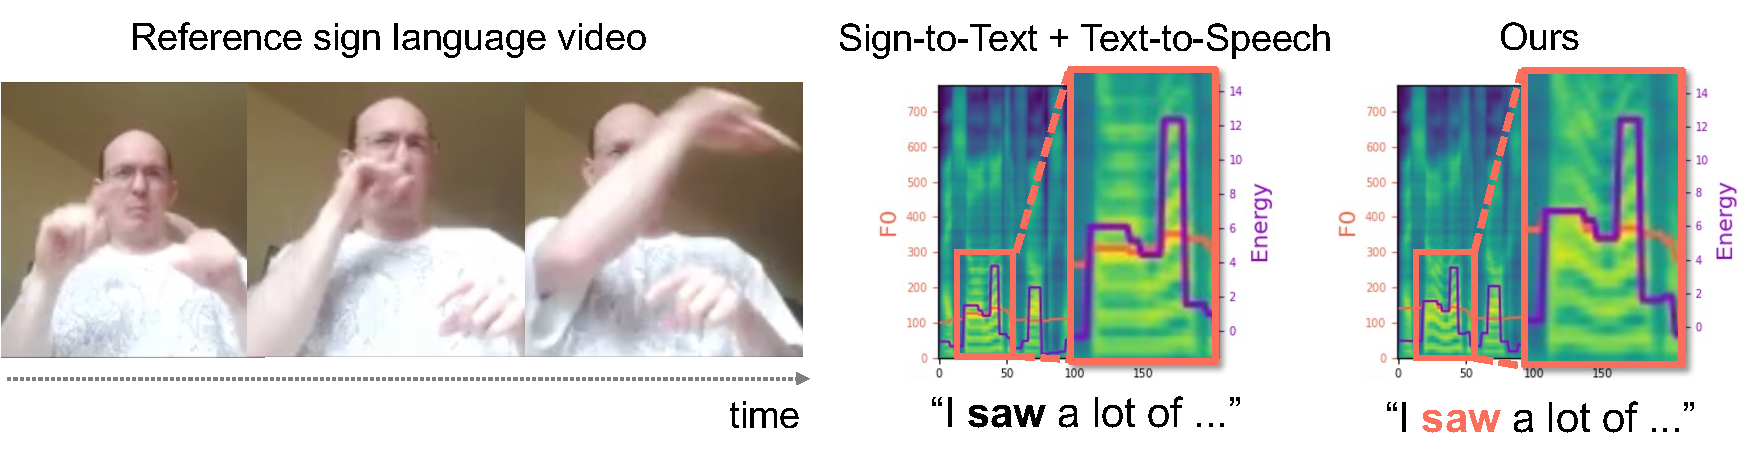
\includegraphics[width=\linewidth]{assets/mel_vis1.pdf}}
    \vspace{-4mm}
    \caption{An example of input sign language video (left) and synthesized speech (right).}
    \vspace{-2mm}
    \label{fig:mel_ex1}
\end{figure}


\subsection{Qualitative Evaluation}
\label{sec:qualitative}
Fig.~\ref{fig:mel_ex1} presents an example of the synthesized speech, one of the highest scored samples in the user study. In the reference sign language video, the signer signs the phrase ``I saw'' with dynamic facial expressions and hand movements. SignRecGAN successfully represents the emphasis on the phrase, while two-stage method fails.

\begin{figure}[th]
    \centering
    \centerline{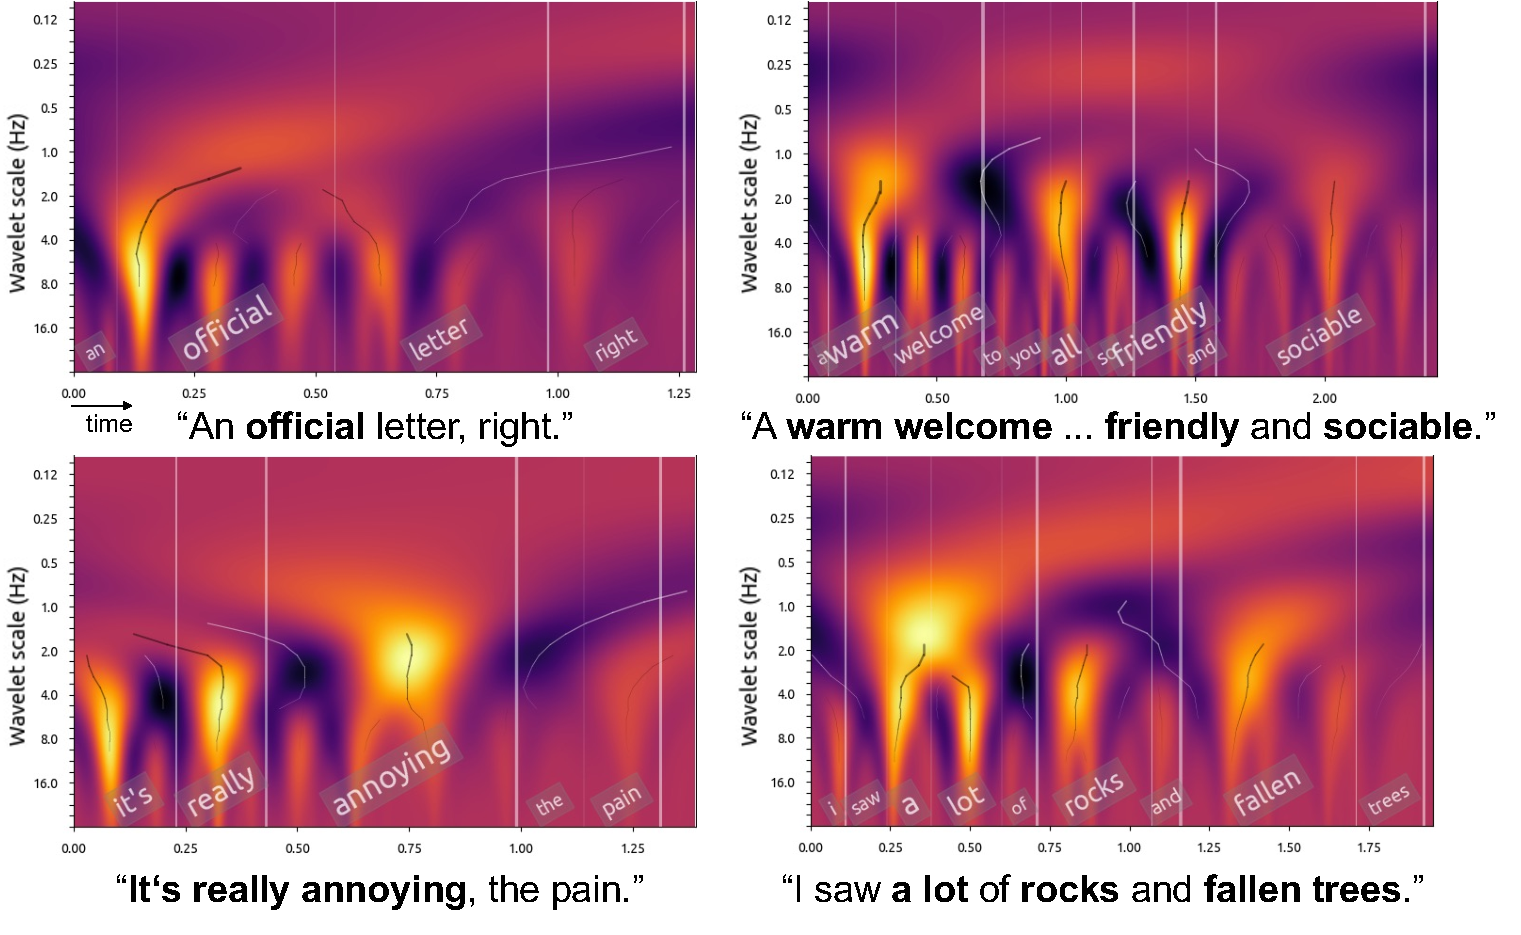
\includegraphics[width=\linewidth]{assets/prominence.pdf}}
    \vspace{-2mm}
    \caption{Prominence analysis results. A black line on a spectrogram indicates emphasis, and the corresponding word is labeled on the spectrogram. The size of a labeled word indicates the intensity of the emphasis.}
    \label{fig:prominece}
    \vspace{-6mm}
\end{figure}

\subsection{Emergence of Emphasis on Natural Words}
\manabe{
Regarding to fine-grained prosody evaluation, Fig.~\ref{fig:prominece} shows some results of prominence analysis~\cite{DBLP:journals/corr/SuniAV15}.
The results indicate that S2PFormer can emphasize suitable words (e.g., ``\textit{annoying}'', ``\textit{a lot}'') and does not emphasize unnatural words (e.g., ``\textit{and}'').
% It is considered to be realized by adversarial learning.
% Therefore, even though SignRecGAN relies on global prosody,
% the synthesized speeches are natural.
This suggests that while the reconstruction loss facilitates the modeling of global prosody, its combination with adversarial learning enables the model to selectively emphasize contextually natural words.
}

% Fig.~\ref{fig:mel_ex2} presents another example of synthesized speech. In this case, the sign language speaker displays particularly expressive facial expressions alongside large, pronounced signing movements. Correspondingly, the resulting speech shows a global increase in both energy and pitch. However, one limitation of the speech synthesized by the proposed method is that the pitch remains nearly constant, leading to an absence of natural intonation. This suggests that, although the ProMo loss effectively aligned the mean values of prosodic features, the SignRec loss may not have been sufficiently trained to capture the overall shape of their distribution.

% \begin{figure}[t]
%     \centering
%     \centerline{\includegraphics[width=0.3\linewidth]{images/melspec/ex2.pdf}}
%     \caption{The reference sign language video and the synthesized speeches of ``Sadly some children never get adopted.''.}
%     \vspace{-2mm}
%     \label{fig:mel_ex2}
% \end{figure}
% \subsection{Limitations}
% \noindent{\bf Emotion understanding:} Because our proposed sign language prosody labels just incorporate lower level metrics such as velocity and acceleration, they may not adequately capture higher level attributes like emotion. We will investigate modeling incorporating richier emotional informatino in future work.

% \noindent{\bf Quantitative evaluation:} Since there is not existing method to measure how the prosody of synthesized speech matches that of sign language, we have to rely on limited aspect of model performance.
